% This text is proprietary.
% It's a part of presentation made by myself.
% It may not used commercial.
% The noncommercial use such as private and study is free
% May 2007
% Author: Sascha Frank 
% University Freiburg 
% www.informatik.uni-freiburg.de/~frank/
%
% 

\documentclass{beamer}
\setbeamertemplate{navigation symbols}{}

\usetheme{Warsaw}

%--------------themes--------------------------

%\usepackage{beamerthemeshadow}
%\setbeamercolor{structure}{fg=gray!90!black}

\usecolortheme{crane} %yellow
\setbeamercolor{structure}{fg=red!90!black} % fg->gradient= start!percentage!end %

% these is to set the bloc colors 

\newenvironment<>{redblock}[1]{%
  \setbeamercolor{block title}{fg=white,bg=red!75!black}%
  \begin{block}#2{#1}}{\end{block}}
  
\newenvironment<>{blueblock}[1]{%
  \setbeamercolor{block title}{fg=white,bg=blue!75!black}%
  \begin{block}#2{#1}}{\end{block}}
  
\newenvironment<>{greenblock}[1]{%
  \setbeamercolor{block title}{fg=white,bg=green!50!black}%
  \begin{block}#2{#1}}{\end{block}}
%--------------- mystuff -----------------------------

%\usepackage{polish}
%\usepackage[polish,main=english]{babel}
\usepackage[utf8]{inputenc}
\usepackage{bm} %bold in math mode
\usepackage{bbold} % math 1 - identity matrix
\usepackage{amsmath,amssymb}
\usepackage{graphicx,subfig} %\usepackage{graphicx,subfigure}
\usepackage{multicol}

\usepackage[
style=numeric, % Citation Style
%style=verbose-trad2, % Citation Style
backend=biber,
natbib=true]{biblatex}
%\usepackage[style=authoryear, backend=biber]{biblatex}
\renewbibmacro{in:}{} % suppress the "In: " before the journaltitle

\hypersetup{urlcolor=blue, colorlinks=true} % Colors hyperlinks in blue - change to black if annoying
\addbibresource{Bibliography.bib}
%--------------- end of mystuff -----------------------------


%add frame numbering
\newcommand*\oldmacro{}%
\let\oldmacro\insertshorttitle%
\renewcommand*\insertshorttitle{%
  \oldmacro\hfill%
  \insertframenumber\,/\,\inserttotalframenumber}
  
%-----------------------------------------------------

\begin{document}
\title{Adjoint Lattice Boltzmann for Optimal Control}  
%\author{Grzegorz Gruszczyński, Łukasz Łaniewski-Wołłk, prof. Jacek Szumbarski}
\author[Grzegorz Gruszczyński]{Grzegorz Gruszczyński\\[3mm] Łukasz Łaniewski-Wołłk, prof. Jacek Szumbarski}
%\date{2016}
\date{\today} 
\institute[*]{
Faculty of Power and Aeronautical Engineering \\
Warsaw University of Technology \\
%City, Province \\[1ex]
%\texttt{e-mail address}
}

\begin{frame}
\titlepage
\end{frame}

\begin{frame}\frametitle{Table of contents}\tableofcontents
\end{frame} 


\section{Introduction} 
\subsection{Motivation}
\begin{frame}\frametitle{Motivation}
    
\begin{redblock}{Goal}
Framework for solving optimal control problems of a discrete dynamical systems in the CFD area. \\
study case: optimal mixing of fluid
\end{redblock}


\pause
\begin{blueblock}{Method}
 \begin{list}{•}{}
  \item Lattice Boltzmann on GPU
  \item Adjoint
  \item Automatic Differentiation
 \end{list}    
\end{blueblock}

%\begin{greenblock}{title of the bloc}
%aaa
%\end{greenblock}


\end{frame}
\subsection{Problem statement}
\begin{frame}\frametitle{Problem statement} 
\begin{figure}
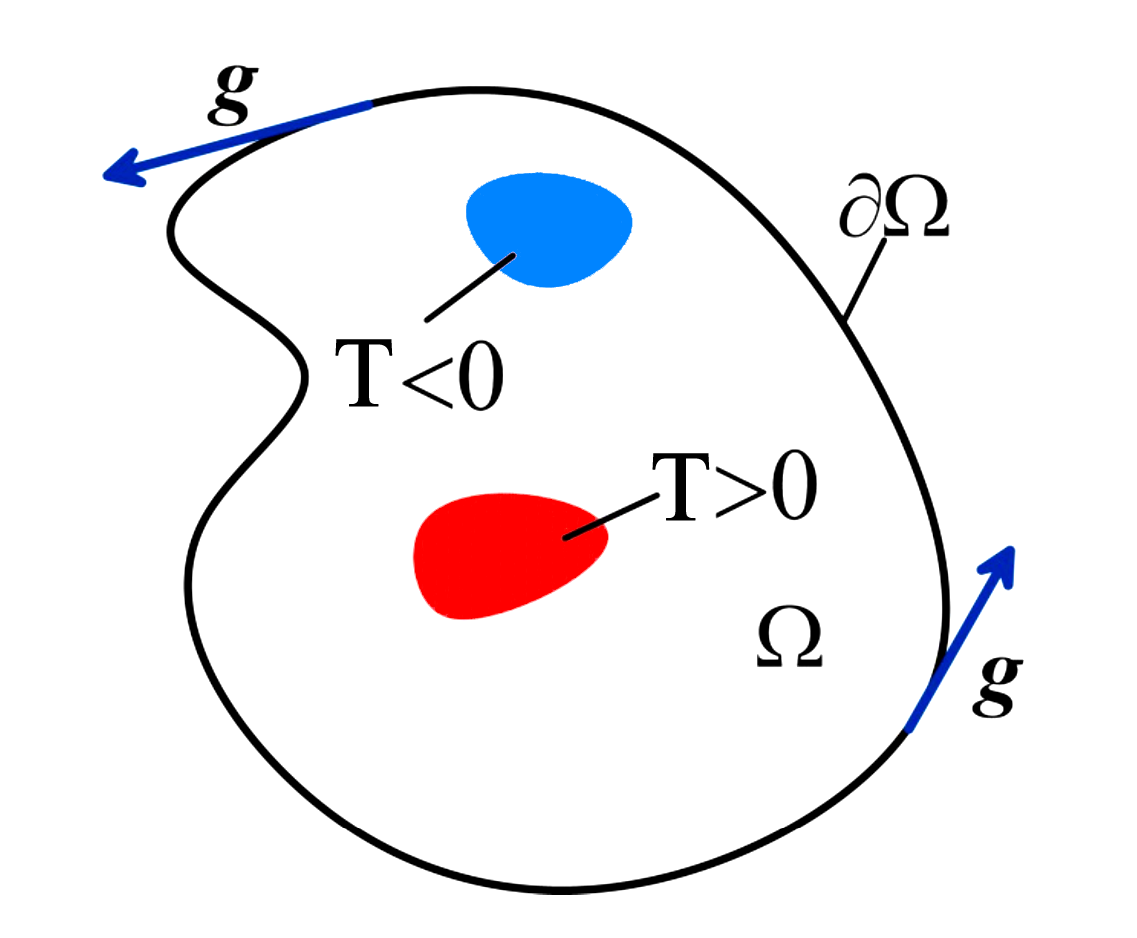
\includegraphics[width = 0.5 \textwidth]{obrazki/FlowDomain_ProblemFormulation.png} 
\caption{Flow Domain}
\end{figure}
\end{frame}


\begin{frame}\frametitle{Fluid Motion} 
\begin{minipage}[c]{0.8\textwidth}
Incompressible Navier Stokes and continuity equation:
\begin{eqnarray}  
\left\{
	\begin{array}{ll}
		\partial_t \boldsymbol{u} + (\boldsymbol{u} \cdot\nabla) \boldsymbol{u} = -\nabla p +\nu \Delta \boldsymbol{u} \\
		\nabla \cdot \boldsymbol{u} = 0
	\end{array}\nonumber 
\right.
\end{eqnarray}

Boundary and Initial Conditions for the fluid:
\begin{eqnarray}  
     \boldsymbol{u} \bigg|_{\partial\Omega} = \boldsymbol{g}
         \hspace{1.5em};\hspace{1.5em} 
     \boldsymbol{g} \cdot \boldsymbol{n}  \bigg|_{\partial\Omega} = 0         		 \hspace{1.5em};\hspace{1.5em} 
     \boldsymbol{u} \bigg|_{t = 0} = 0 \nonumber
\end{eqnarray} 
\end{minipage}\hfill
\begin{minipage}[c]{0.2\textwidth} % use [c], [t] or [b] for vertical alignment
   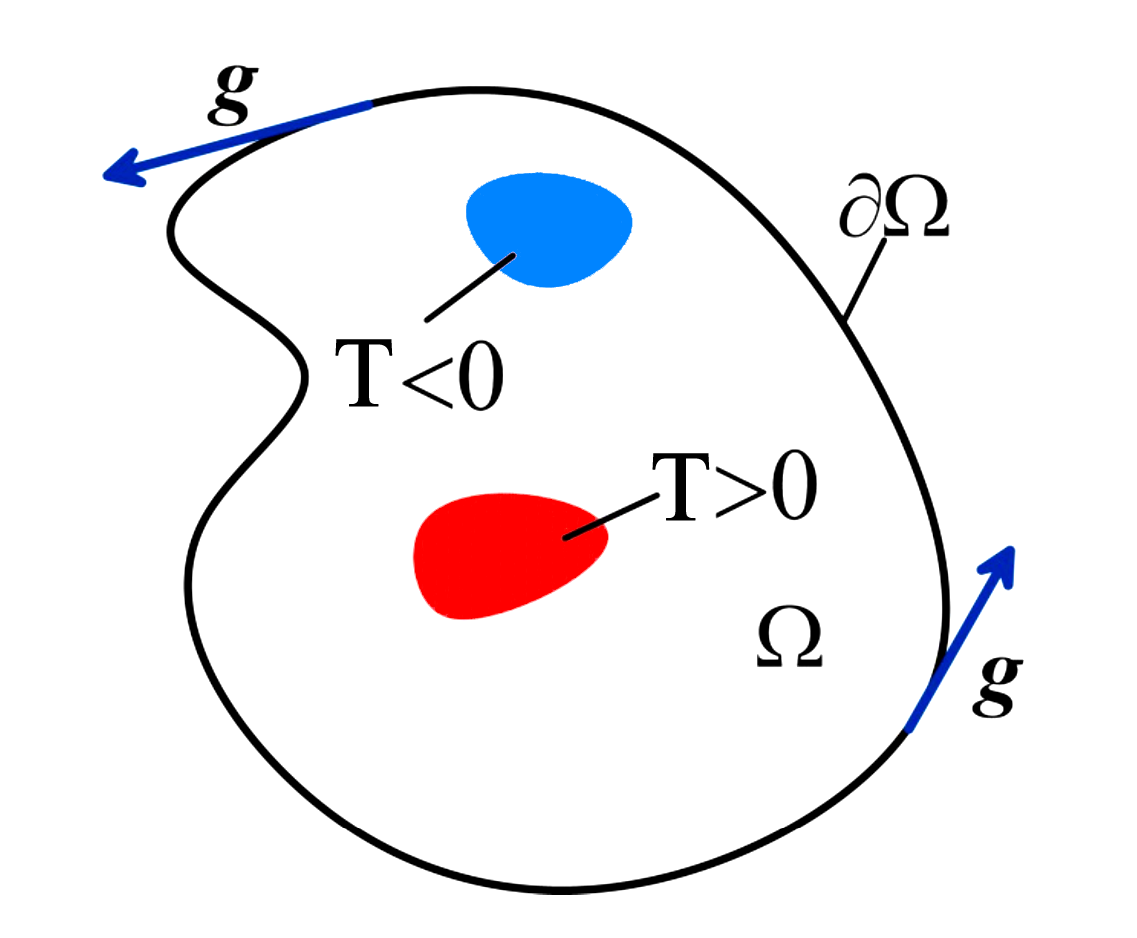
\includegraphics[width = 1.5 \textwidth]
   {obrazki/FlowDomain_ProblemFormulation.png} 
\end{minipage}
\end{frame}


\begin{frame} \frametitle{Passive Scalar} 
\begin{minipage}[c]{0.8\textwidth}
Advection - diffusion equation:
\begin{eqnarray}
\partial_t T +  \boldsymbol{u} \cdot \nabla T = \lambda \nabla^2 T \nonumber
\end{eqnarray}
%\pause 
Boundary and Initial Conditions for the Passive Scalar:
\begin{eqnarray}  
       \frac{\partial}{\partial \boldsymbol{n}}  T \bigg|_{\partial \Omega} = 0 
       \hspace{1.5em};\hspace{1.5em} 
       T \bigg|_{t = 0} = T_0 \nonumber
\end{eqnarray}
\end{minipage}\hfill
\begin{minipage}[c]{0.2\textwidth} % use [c], [t] or [b] for vertical alignment
   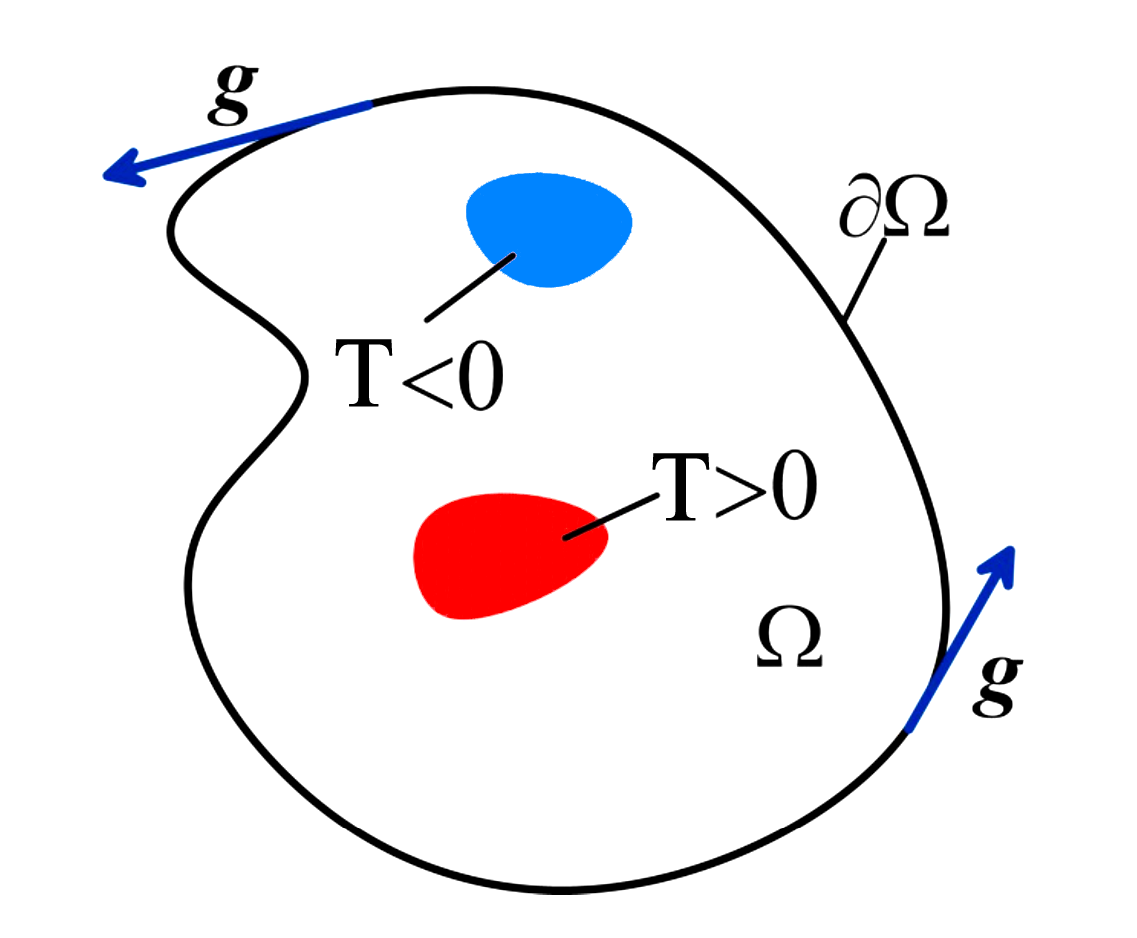
\includegraphics[width = 1.5 \textwidth]
   {obrazki/FlowDomain_ProblemFormulation.png} 
\end{minipage}

\end{frame}


\begin{frame} \frametitle{Objective function} 
Find an extremum of the functional:
\begin{eqnarray}  
J[\bm{u},T] = \underbrace{ \int_{\Omega} [T(t_{end}) - \overline{T} ]^2 d\bm{x} }_{\text{$I_1$ - mix quality}} + 
 \varepsilon \underbrace{\bigg[\int_{0}^{t_{end}} \bigg(\int_{\partial\Omega} 2\nu \bm{u}  \cdot \bm{D_u} \bm{n} dS  \bigg)dt  \bigg]^2}_{\text{$I_2$ - work needed to impose motion}} \nonumber
\end{eqnarray}
where: 
\begin{eqnarray}
			\bm{D_u} = \frac{1}{2} ( \nabla \bm{u}  + \nabla^T \bm{u} )  \hspace{3em} 
				&-& \text{deformation rate tensor} \nonumber \\
			\overline{T} = \frac{1}{|\Omega|} \int_{\Omega} T d\bm{x} \hspace{3em}
				&-& \text{average value of the passive scalar} \nonumber \\
			\varepsilon   \hspace{3em}
				&-& \text{ weight coefficient} \nonumber
\end{eqnarray} 

\end{frame}
 
 
\section{Lattice Boltzmann Method} 
\subsection{Algorithm}
%\subsection{Boltzmann equation}
%\begin{frame}\frametitle{The Boltzmann transport equation}
% 
%\begin{eqnarray} \label{Boltzmann_equation}
%	\dfrac{\partial f}{\partial t} + (\textbf{u} \cdot \nabla) f = \mathbb{C}(f) \nonumber
%\end{eqnarray}
%
%\begin{itemize}
%\item $f(\bm{x}, t )$ - particle distribution function
%\item $\bm{u}$ - particle velocity
%\item $\mathbb{C}(f)$ - collision operator
%\end{itemize}
%\end{frame} 

\begin{frame}\frametitle{ The Lattice Boltzmann equation}
\begin{eqnarray} \label{DiscretizedBoltzmannEquation}
	 \underbrace{ f_i(\bm{x}+ \bm{e_i} \Delta {\bm{x}}, t +  \Delta {t} ) - f_i(\bm{x}, t )}_{Streaming} =
  \underbrace{ - \frac{1}{\tau } ( f_i - f_i^{eq})}_{Collision} \nonumber
\end{eqnarray}
\begin{itemize}
\item $\tau$ - relaxation parameter, $\tau = 3\nu \dfrac{(\Delta x)^2}{\Delta t} + \dfrac{1}{2}$ where $\nu$ is the kinematic viscosity 
\item $f_i$ - discrete probability distribution function
\end{itemize}
\begin{figure}
  \begin{minipage}[c]{0.6\textwidth}
    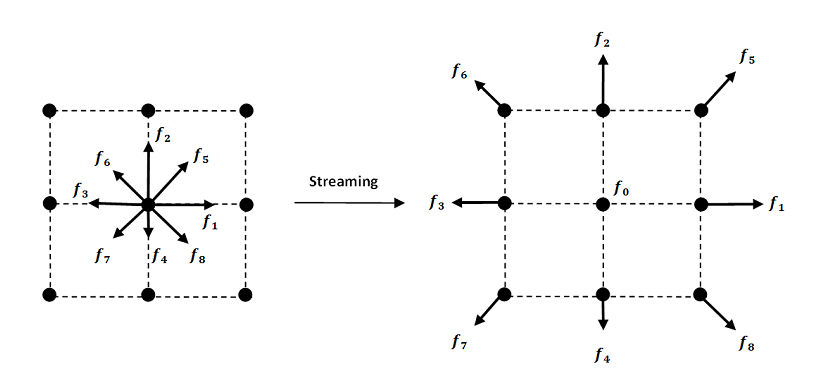
\includegraphics[width=\textwidth]{obrazki/streaming.png} 
  \end{minipage}\hfill
  \begin{minipage}[c]{0.4\textwidth} % use [c], [t] or [b] for vertical alignment
    \caption{D2Q9: Streaming} \label{fig:Streaming}
  \end{minipage}
\end{figure}

%\begin{figure}
%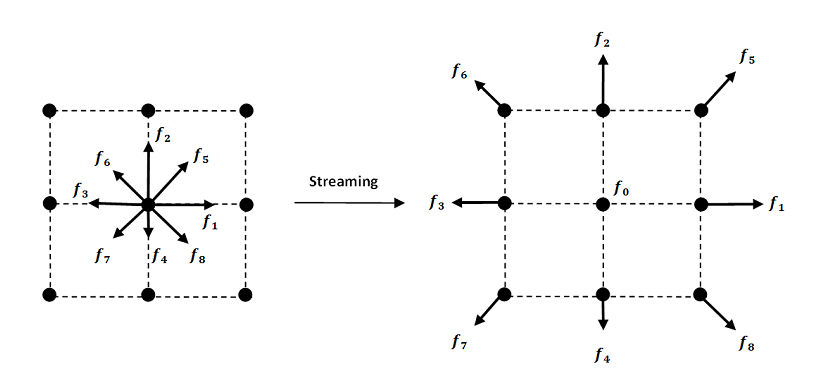
\includegraphics[width =0.6 \textwidth]{obrazki/streaming.png} 
%%\caption{Streaming}
%\end{figure}

\end{frame} 
 

\begin{frame}[plain] \frametitle{Algorithm: Fluid} 
\textit{1} Initialize $ %\rho, \enspace \boldsymbol{u}(\boldsymbol{x},t), \enspace f_i ^{eq}
 \enspace f_i ^{in} $ \newline

\pause
\textit{2} Compute $ \rho, \enspace \boldsymbol{u}(\boldsymbol{x},t) $
\begin{eqnarray}  
         \rho = \sum_{i=0}^{8} f_i ^{in}(\boldsymbol{x},t)
          \hspace{2em}  and  \hspace{2em}
      	 \boldsymbol{u}(\boldsymbol{x},t) =  \dfrac{1}{\rho} \sum_{i=0}^{8} \, f_i ^{in}(\boldsymbol{x},t) \boldsymbol{e}_i  \nonumber  
\end{eqnarray}

\pause
\textit{3} Compute $ f_i ^{eq}(\boldsymbol{x},t)$
\begin{eqnarray}   
 f_i ^{eq}(\boldsymbol{x},t) = w_i \rho(\boldsymbol{x},t) 
 \left[ 1+ 3 \frac{\boldsymbol{e}_i \boldsymbol{u}}{e^2} +\frac{9}{2} \frac{ (\boldsymbol{e}_i \boldsymbol{u})^2}{e^4} - \frac{3}{2} \frac{\boldsymbol{u}^2 } {e^2} \right]    \nonumber  
\end{eqnarray}

\pause
\textit{4} BGK Collision
\begin{eqnarray}   
 f_i ^{out}(\boldsymbol{x},t) = f_i^{in}(\boldsymbol{x},t) - \frac{1}{\tau_f} \bigg( f_i^{in}(\boldsymbol{x},t) - f_i^{eq}(\boldsymbol{x},t) \bigg)\nonumber  
 % (1 -  \frac{1}{\tau_f}) f_i^{in} (\boldsymbol{x},t)  +  \Omega_f f_i^{eq} (\boldsymbol{x},t) \nonumber  
\end{eqnarray}

\pause
\textit{5} Streaming
\begin{eqnarray}   
 f_i ^{in}(\boldsymbol{x} + \boldsymbol{e}_i ,t+1) =  f_i^{out} (\boldsymbol{x},t) \nonumber  
\end{eqnarray}

\end{frame} 


% \subsection{Algorithm}
\begin{frame}[plain]\frametitle{Algorithm: Passive Scalar}

Advection - Diffusion of the T is solved on a separate D2Q5 lattice \newline

\textit{1} Initialize $ \theta_i ^{in} (\boldsymbol{x},t) $ \newline

%\pause
\textit{2} Compute $  T(\boldsymbol{x},t) $
\begin{eqnarray}  
         T(\boldsymbol{x},t) = \sum_{i=0}^{4} \theta_i ^{in}(\boldsymbol{x},t) \nonumber
\end{eqnarray}

%\pause
\textit{3} Compute $ \theta_i ^{eq}(\boldsymbol{x},t)$
\begin{eqnarray}   
 \theta_i ^{eq}(\boldsymbol{x},t) = T(\boldsymbol{x},t) w_i 
 \left[ 1+ 3 \frac{\boldsymbol{e}_i \boldsymbol{u}}{e^2}  \right]    \nonumber  
\end{eqnarray}

%\pause
\textit{4} BGK Collision
\begin{eqnarray}   
\theta_i ^{out}(\boldsymbol{x},t) = \theta_i^{in}(\boldsymbol{x},t) - \frac{1}{\tau_T} \bigg( \theta_i^{in}(\boldsymbol{x},t) - \theta_i^{eq}(\boldsymbol{x},t) \bigg)\nonumber
 %T_i ^{out}(\boldsymbol{x},t) = (1 - \Omega_T) T_i^{in} (\boldsymbol{x},t)  +  \Omega_T T_i^{eq} (\boldsymbol{x},t) \nonumber  
\end{eqnarray}

%\pause
\textit{5} Streaming
\begin{eqnarray}   
 \theta_i ^{in}(\boldsymbol{x} + \boldsymbol{e}_i ,t+1) =  \theta_i^{out} (\boldsymbol{x},t) \nonumber  
\end{eqnarray}
\end{frame} 


\subsection{Validation}  
\begin{frame}\frametitle{Validation}
\begin{itemize}
\item flow - frequency of shedding of von Karman vortices
\item advection	
\item diffusion
\item passive scalar conservation
\item wall shear force - Couette flow
\end{itemize}
\begin{figure}
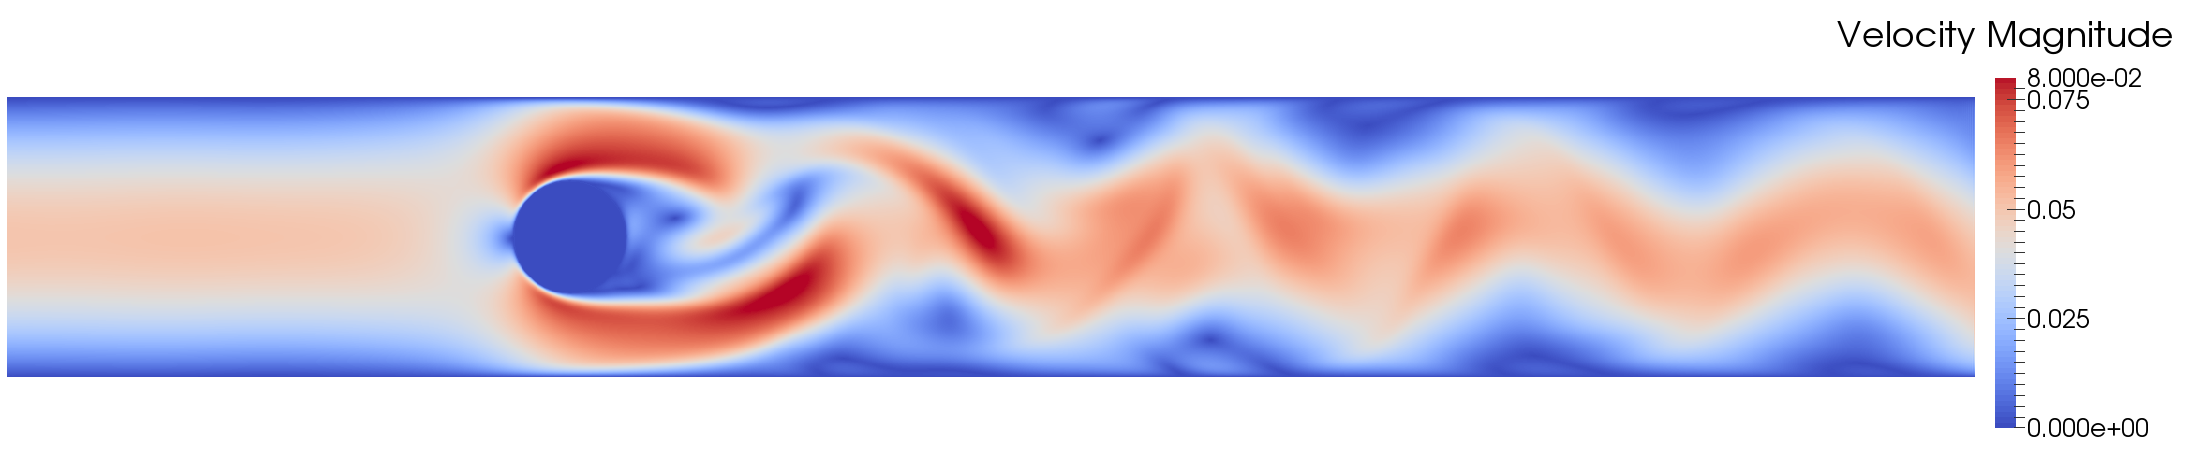
\includegraphics[width =1 \textwidth]{obrazki/karman_snapshot.png} 
%\caption{Streaming}
\end{figure}

%\vspace{-2em}
%
%\begin{figure}[H]
%\centering     %%% not \center
%\subfloat{
%\includegraphics[width=0.5 \textwidth]
%{obrazki/KarmanSignal.jpg}}%\par
%\subfloat{
%\includegraphics[width=0.5 \textwidth]
%{obrazki/UniformlyDistributedPassiveScalar.png}}
%
%\subfloat{
%\includegraphics[width=0.5 \textwidth]
%{obrazki/advection.png}}
%\subfloat{
%\includegraphics[width=0.5 \textwidth]
%{obrazki/diffusion.png}}
%
%%\caption{History of passive scalar (left) and velocity (right) fields}%\label{fig:animals}
%\end{figure}

\end{frame} 
 
\section{Adjoint for LBM} 
\subsection{General concept}
\begin{frame}\frametitle{Why adjoint?}
Primal equation
\begin{eqnarray}  
       Au = b \nonumber
\end{eqnarray}

\uncover<2->{
Dual equation
\begin{eqnarray}  
       A^T v = h \nonumber
\end{eqnarray}
}

Find the value of a functional $ h\cdot u $
\begin{eqnarray}  
      h^T u = \uncover<2->{(A^T v)^T u = v^T \underbrace{Au}_{b} = v^T b } \nonumber
\end{eqnarray}

\end{frame} 

\subsection{Application to LBM}
%\begin{frame}\frametitle{Discrete dynamical system}
\begin{frame}[plain]\frametitle{Discrete dynamical system}
\begin{equation}
\label{primal}
     \begin{bmatrix}
         u_{n+1} \\
         g_{n+1} 
        \end{bmatrix} 
        = H ( u_n, \alpha_n) \nonumber
         \uncover<3->{
         \xrightarrow[]{adjoint}
    \begin{bmatrix}
         v_{n-1} \\
         \beta_{n-1} 
     \end{bmatrix} 
        = [dH]^T 
     \begin{bmatrix}
         v_{n} \\
         h_{n} 
     \end{bmatrix} \nonumber
     }
\end{equation}
\vspace{-2ex}
\begin{figure}[H]
\begin{center}
   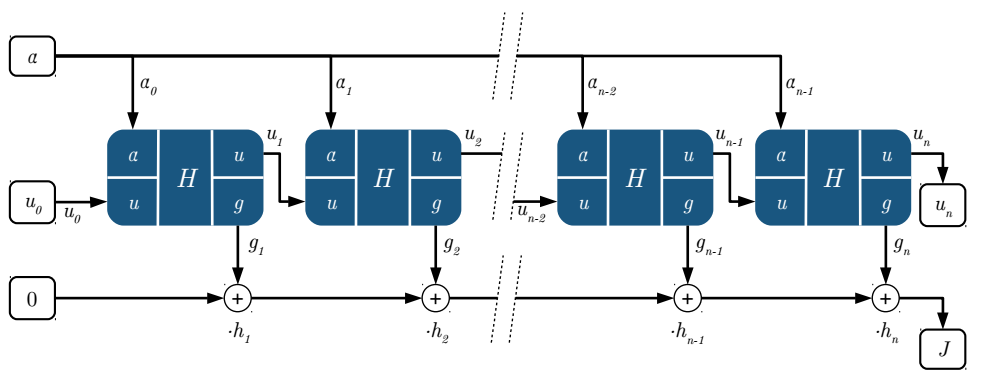
\includegraphics[width= 0.9 \textwidth]{obrazki/dynamicIterativeProcess.png} 
    \caption[Discrete iterative process]{Discrete iterative process (from \citet*{phd_laniewski})}
 \end{center}
\end{figure}
\uncover<2->{
Find the derivative of the objective $J = \textbf{h} \cdot \textbf{g} $ with respect to a formal differentiation parameter $s$:
\begin{eqnarray}  
  \frac{d}{ds} J =  \frac{d}{ds} (\textbf{h} \cdot \textbf{g}) =  \sum_{n=1}^{N} h_n \cdot \dfrac{\partial g_n}{\partial s} 
  \uncover<3->{ \xrightarrow[]{adjoint}
   v_0 \cdot \frac{\partial u_0}{\partial s} + \sum_{n=0}^{N-1} \beta_n \cdot \dfrac{\partial \alpha_n}{\partial s}
  }
  \nonumber
\end{eqnarray}
}
\end{frame} 


\begin{frame}[plain]\frametitle{The primal $ \rightarrow $ adjoint formulation:}

\begin{equation}
     \begin{bmatrix}
         u_{n+1} \\
         g_{n+1} 
        \end{bmatrix} 
        = H ( u_n, \alpha_n) \xrightarrow[]{adjoint}
    \begin{bmatrix}
         v_{n-1} \\
         \beta_{n-1} 
     \end{bmatrix} 
        = [dH]^T 
     \begin{bmatrix}
         v_{n} \\
         h_{n} 
     \end{bmatrix} \nonumber
\end{equation}
\begin{figure}[H]
	\begin{center}
   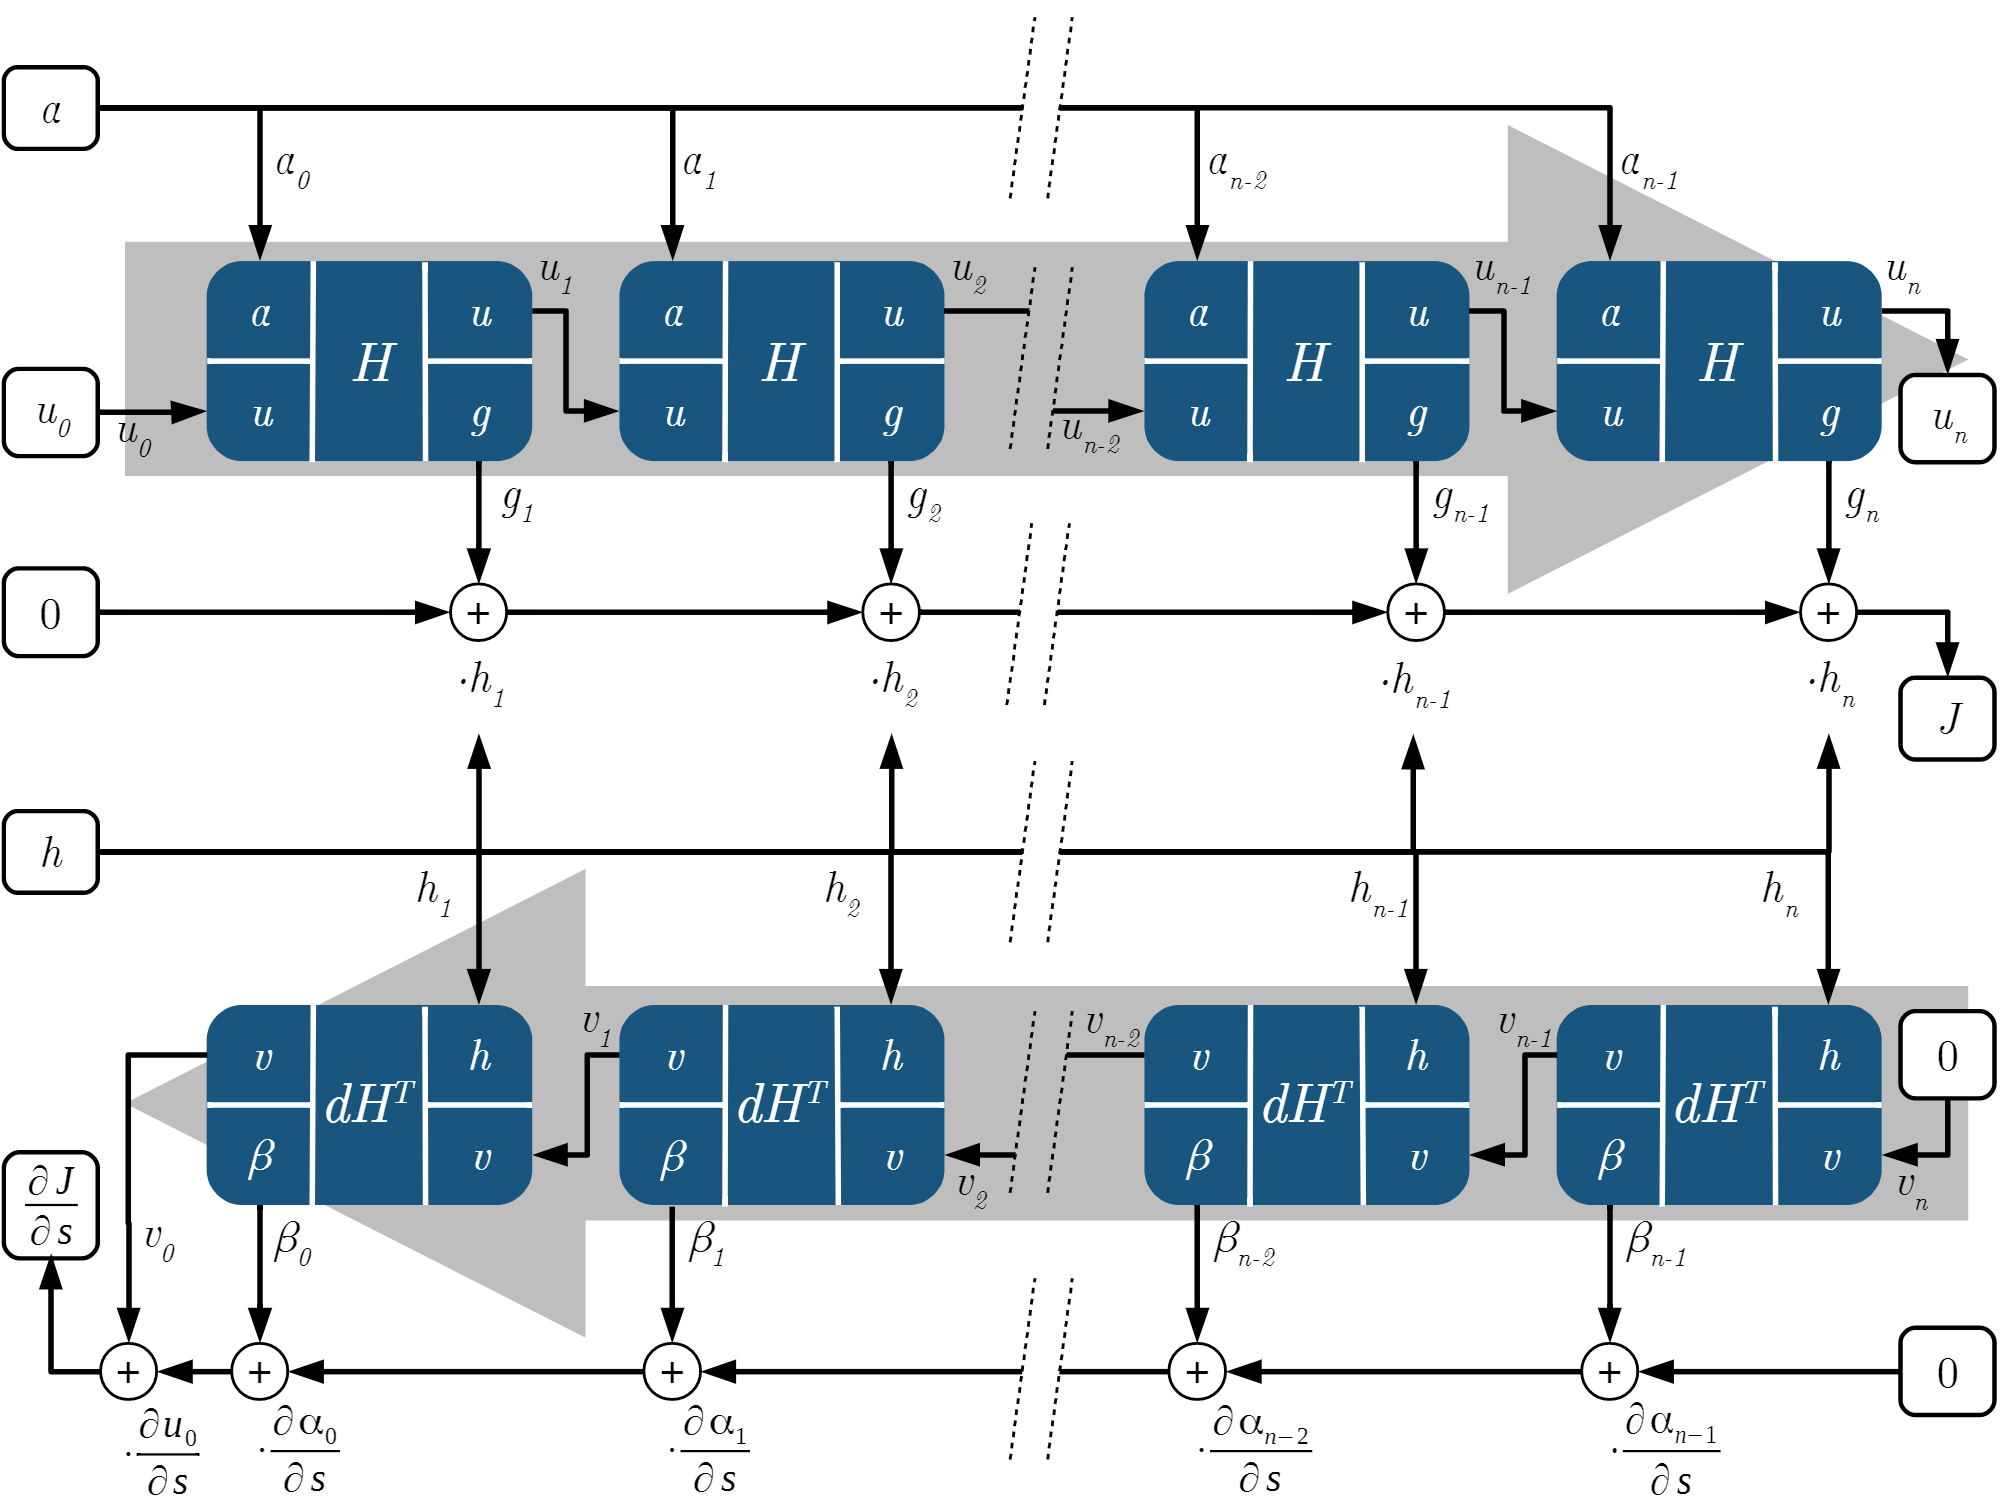
\includegraphics[width= 0.9 \textwidth]{obrazki/adJoint.png} 
   %\caption[Discrete adjoint iterative process]{Discrete adjoint iterative process}
 	\end{center}
\end{figure}

\end{frame} 

\subsection{Automatic differentiation}
\begin{frame}\frametitle{Automatic differentiation}

To compute the derivatives the automatic differentiation is used.
Automatic differentiation is not:
\begin{itemize}
\item Symbolic differentiation
\item Numerical differentiation (the method of finite differences)
\end{itemize}
\pause
\begin{figure}[H]
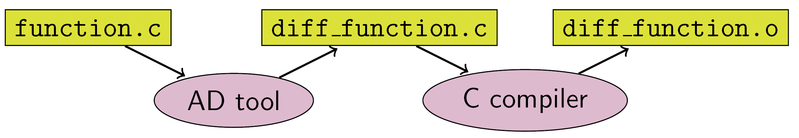
\includegraphics[width=1 \textwidth]{obrazki/SourceTransformationAutomaticDifferentiation.png} 
\caption{Source Code Transformation}
\end{figure}
\end{frame}

\section{Summary} 
\subsection{Results}
\begin{frame}\frametitle{Study case - lid driven cavity}
\begin{figure}[H]
\begin{center}
   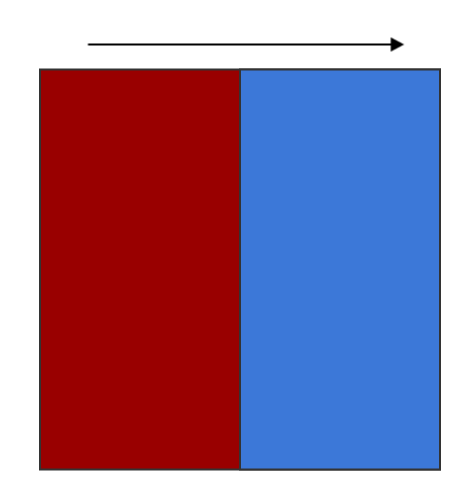
\includegraphics[width= 0.25 \textwidth]{obrazki/IC.png} 
   \caption{Initial conditions for the passive scalar distribution, fluid is at rest}
   %\label{fig:blabal}
 \end{center}
\end{figure}
\begin{itemize}
\item Reference control function: $ U_{lid} = 0.1 \, sin(t)$ and $ t \in [0, 2\pi] $ 
\item Lattice size (with walls): 128x128
\item Lattice fluid viscosity : $\nu = 0.1 $
\item Lattice fluid thermal diffusivity: $\lambda = 0.005 $
\item passive scalar intensity: half domain $ \pm 1$ $\Rightarrow$ average  $ \overline{T} = 0 $
\end{itemize}
\end{frame}

\begin{frame}\frametitle{Study case - results}
\begin{multicols}{2}
\begin{figure}[H]
\begin{center}
   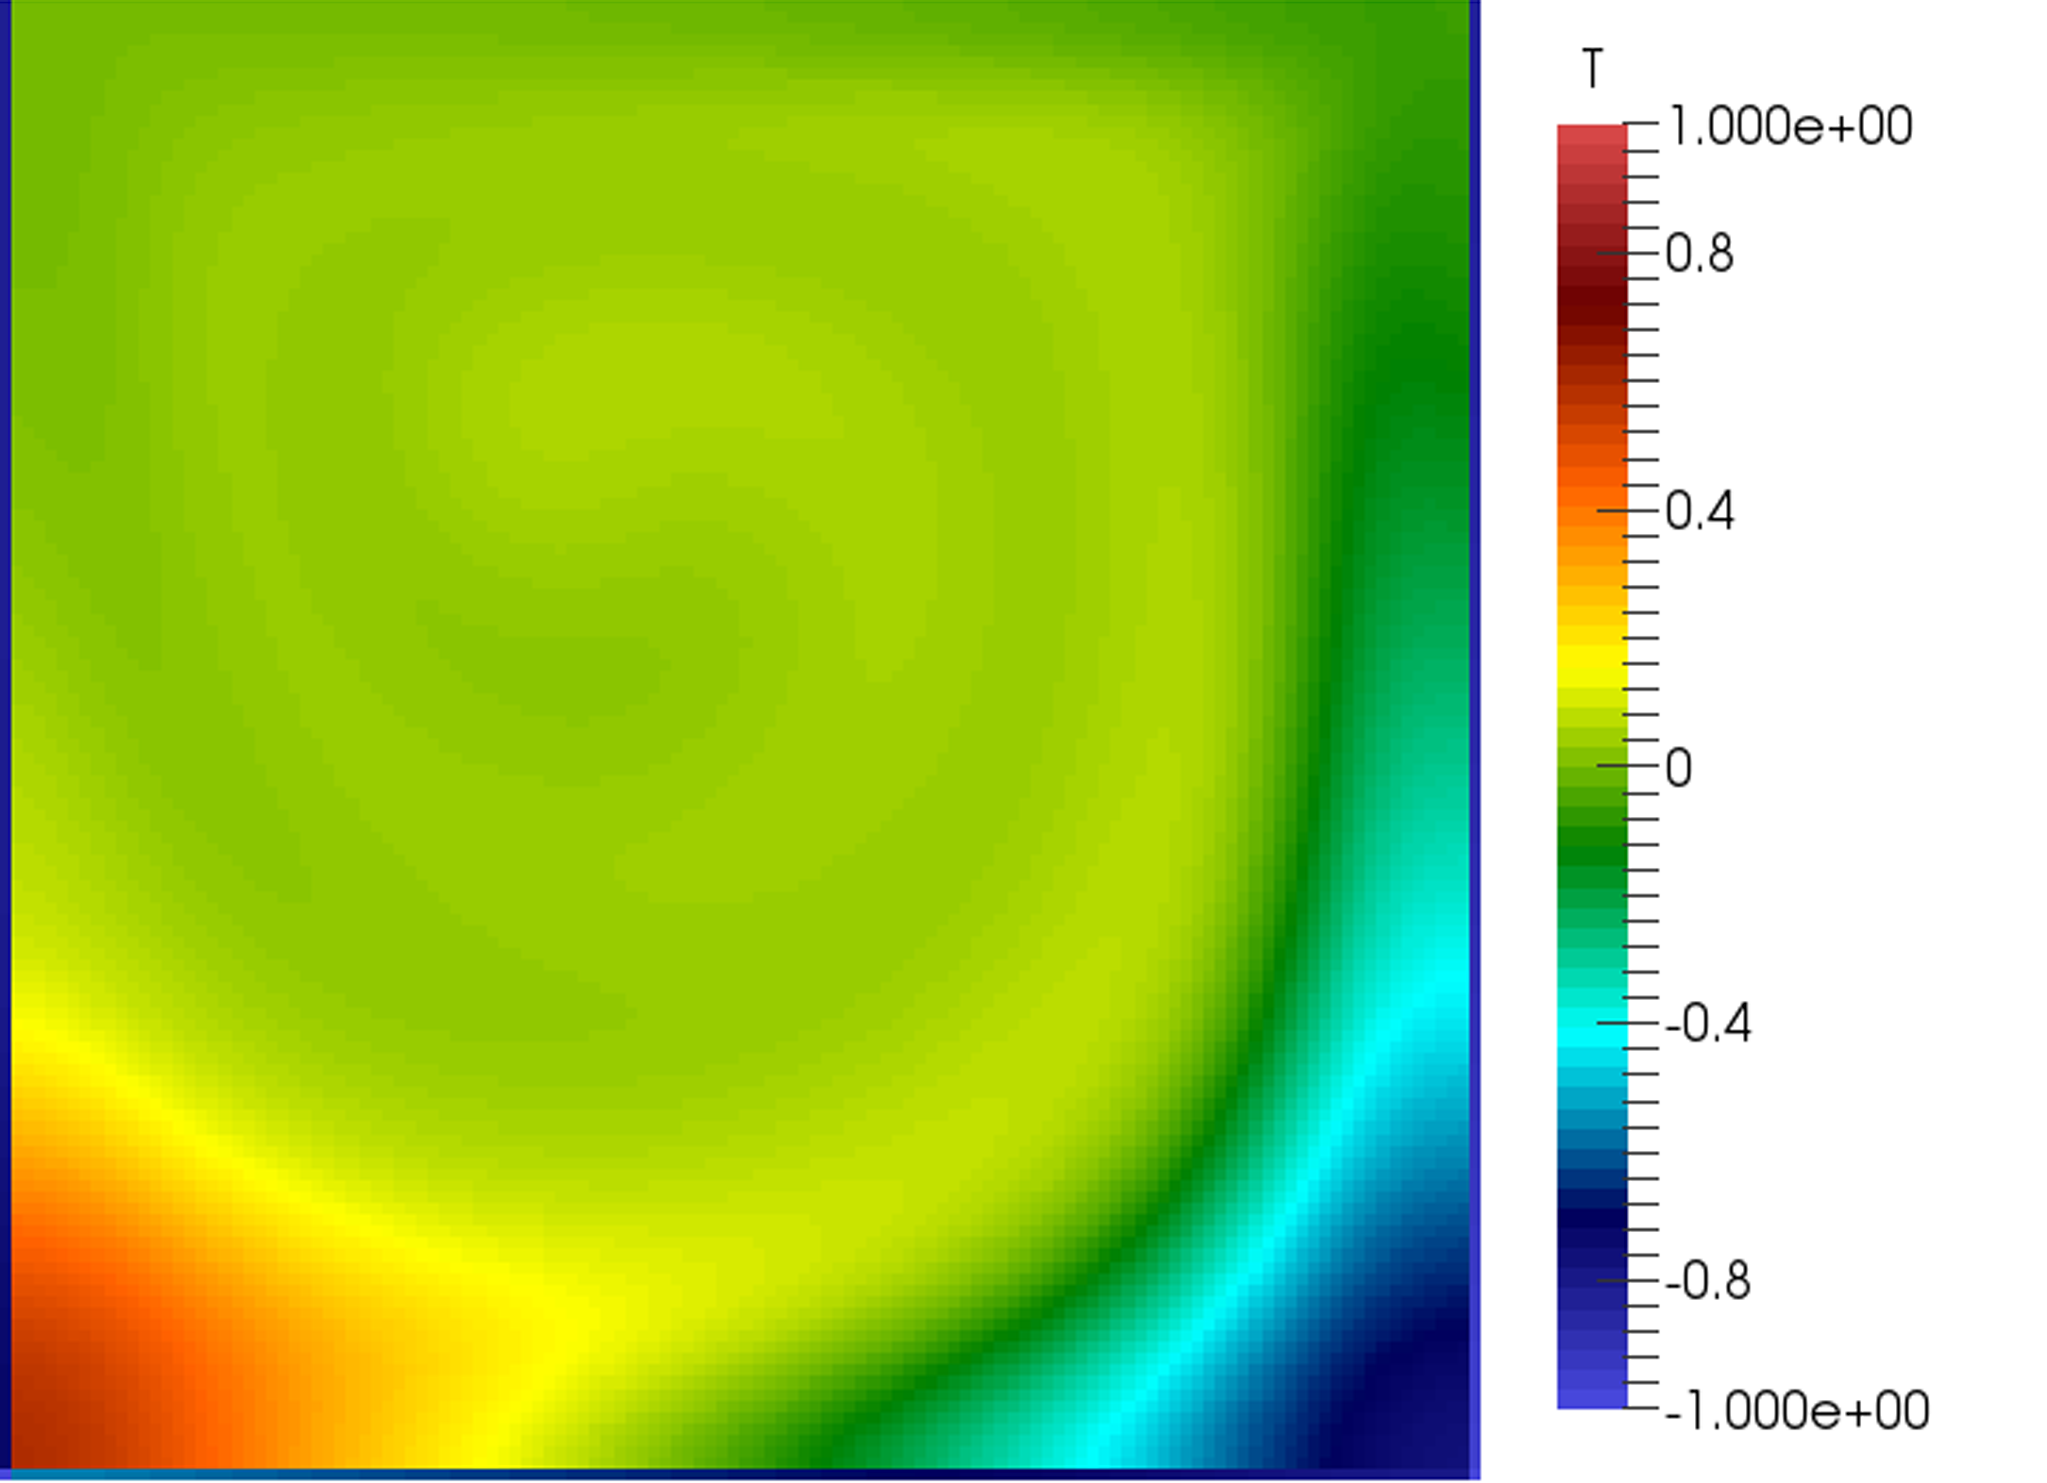
\includegraphics[width= 0.45 \textwidth]{obrazki/T_50k_eps1E_5_1iter.png} 
   \caption{Initial control}
   %\label{fig:blabal}
 \end{center}
\end{figure}
\columnbreak 
\begin{figure}[H]
\begin{center}
   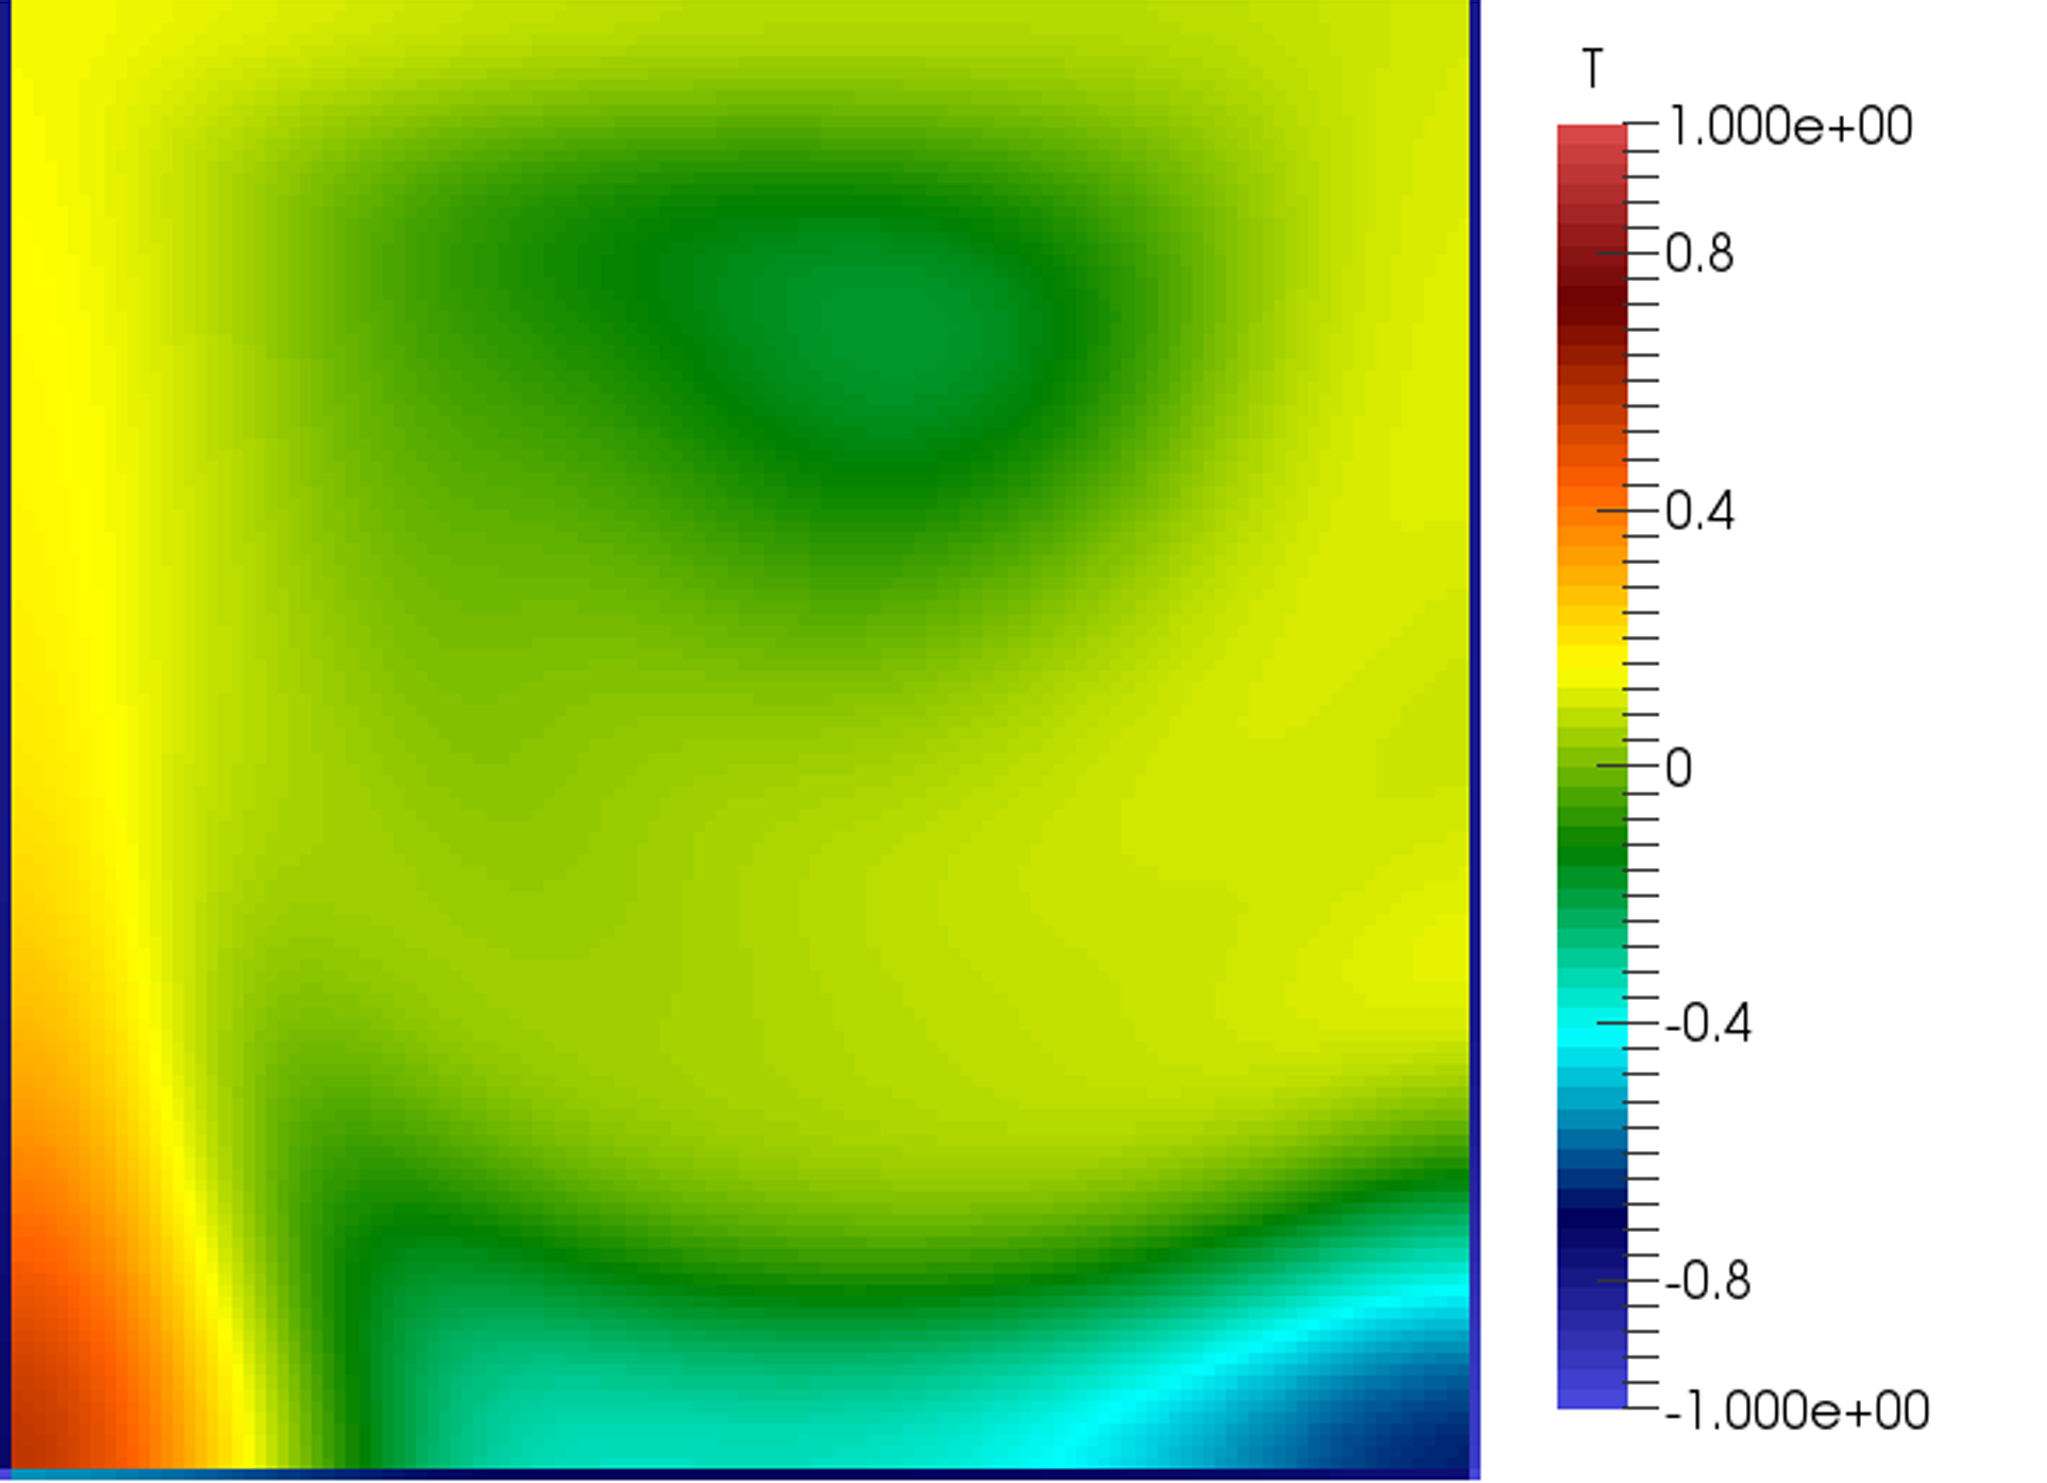
\includegraphics[width= 0.45 \textwidth]{obrazki/T_50k_eps1E_5_opt.png} 
   \caption{Optimized control}
   %\label{fig:blabal}
 \end{center}
\end{figure}
\end{multicols}

\vspace{-5ex}
\begin{center}
\begin{tabular}{|c|c|c|c|c|}
\hline
 			& \textbf{mix quality} 	& \textbf{work} &  \textbf{$\epsilon$ - work weight} & \textbf{J} \\ \hline
initial control  	 & 0.032 		&  9536 		& 1E-5				   & 0.127 		\\ \hline
optimized control	 & 0.025		&  3873 		& 1E-5				   & 0.064		\\ \hline
\end{tabular}
\end{center}
 
\end{frame}

\begin{frame}\frametitle{Pareto Frontier}
\begin{figure}[H]
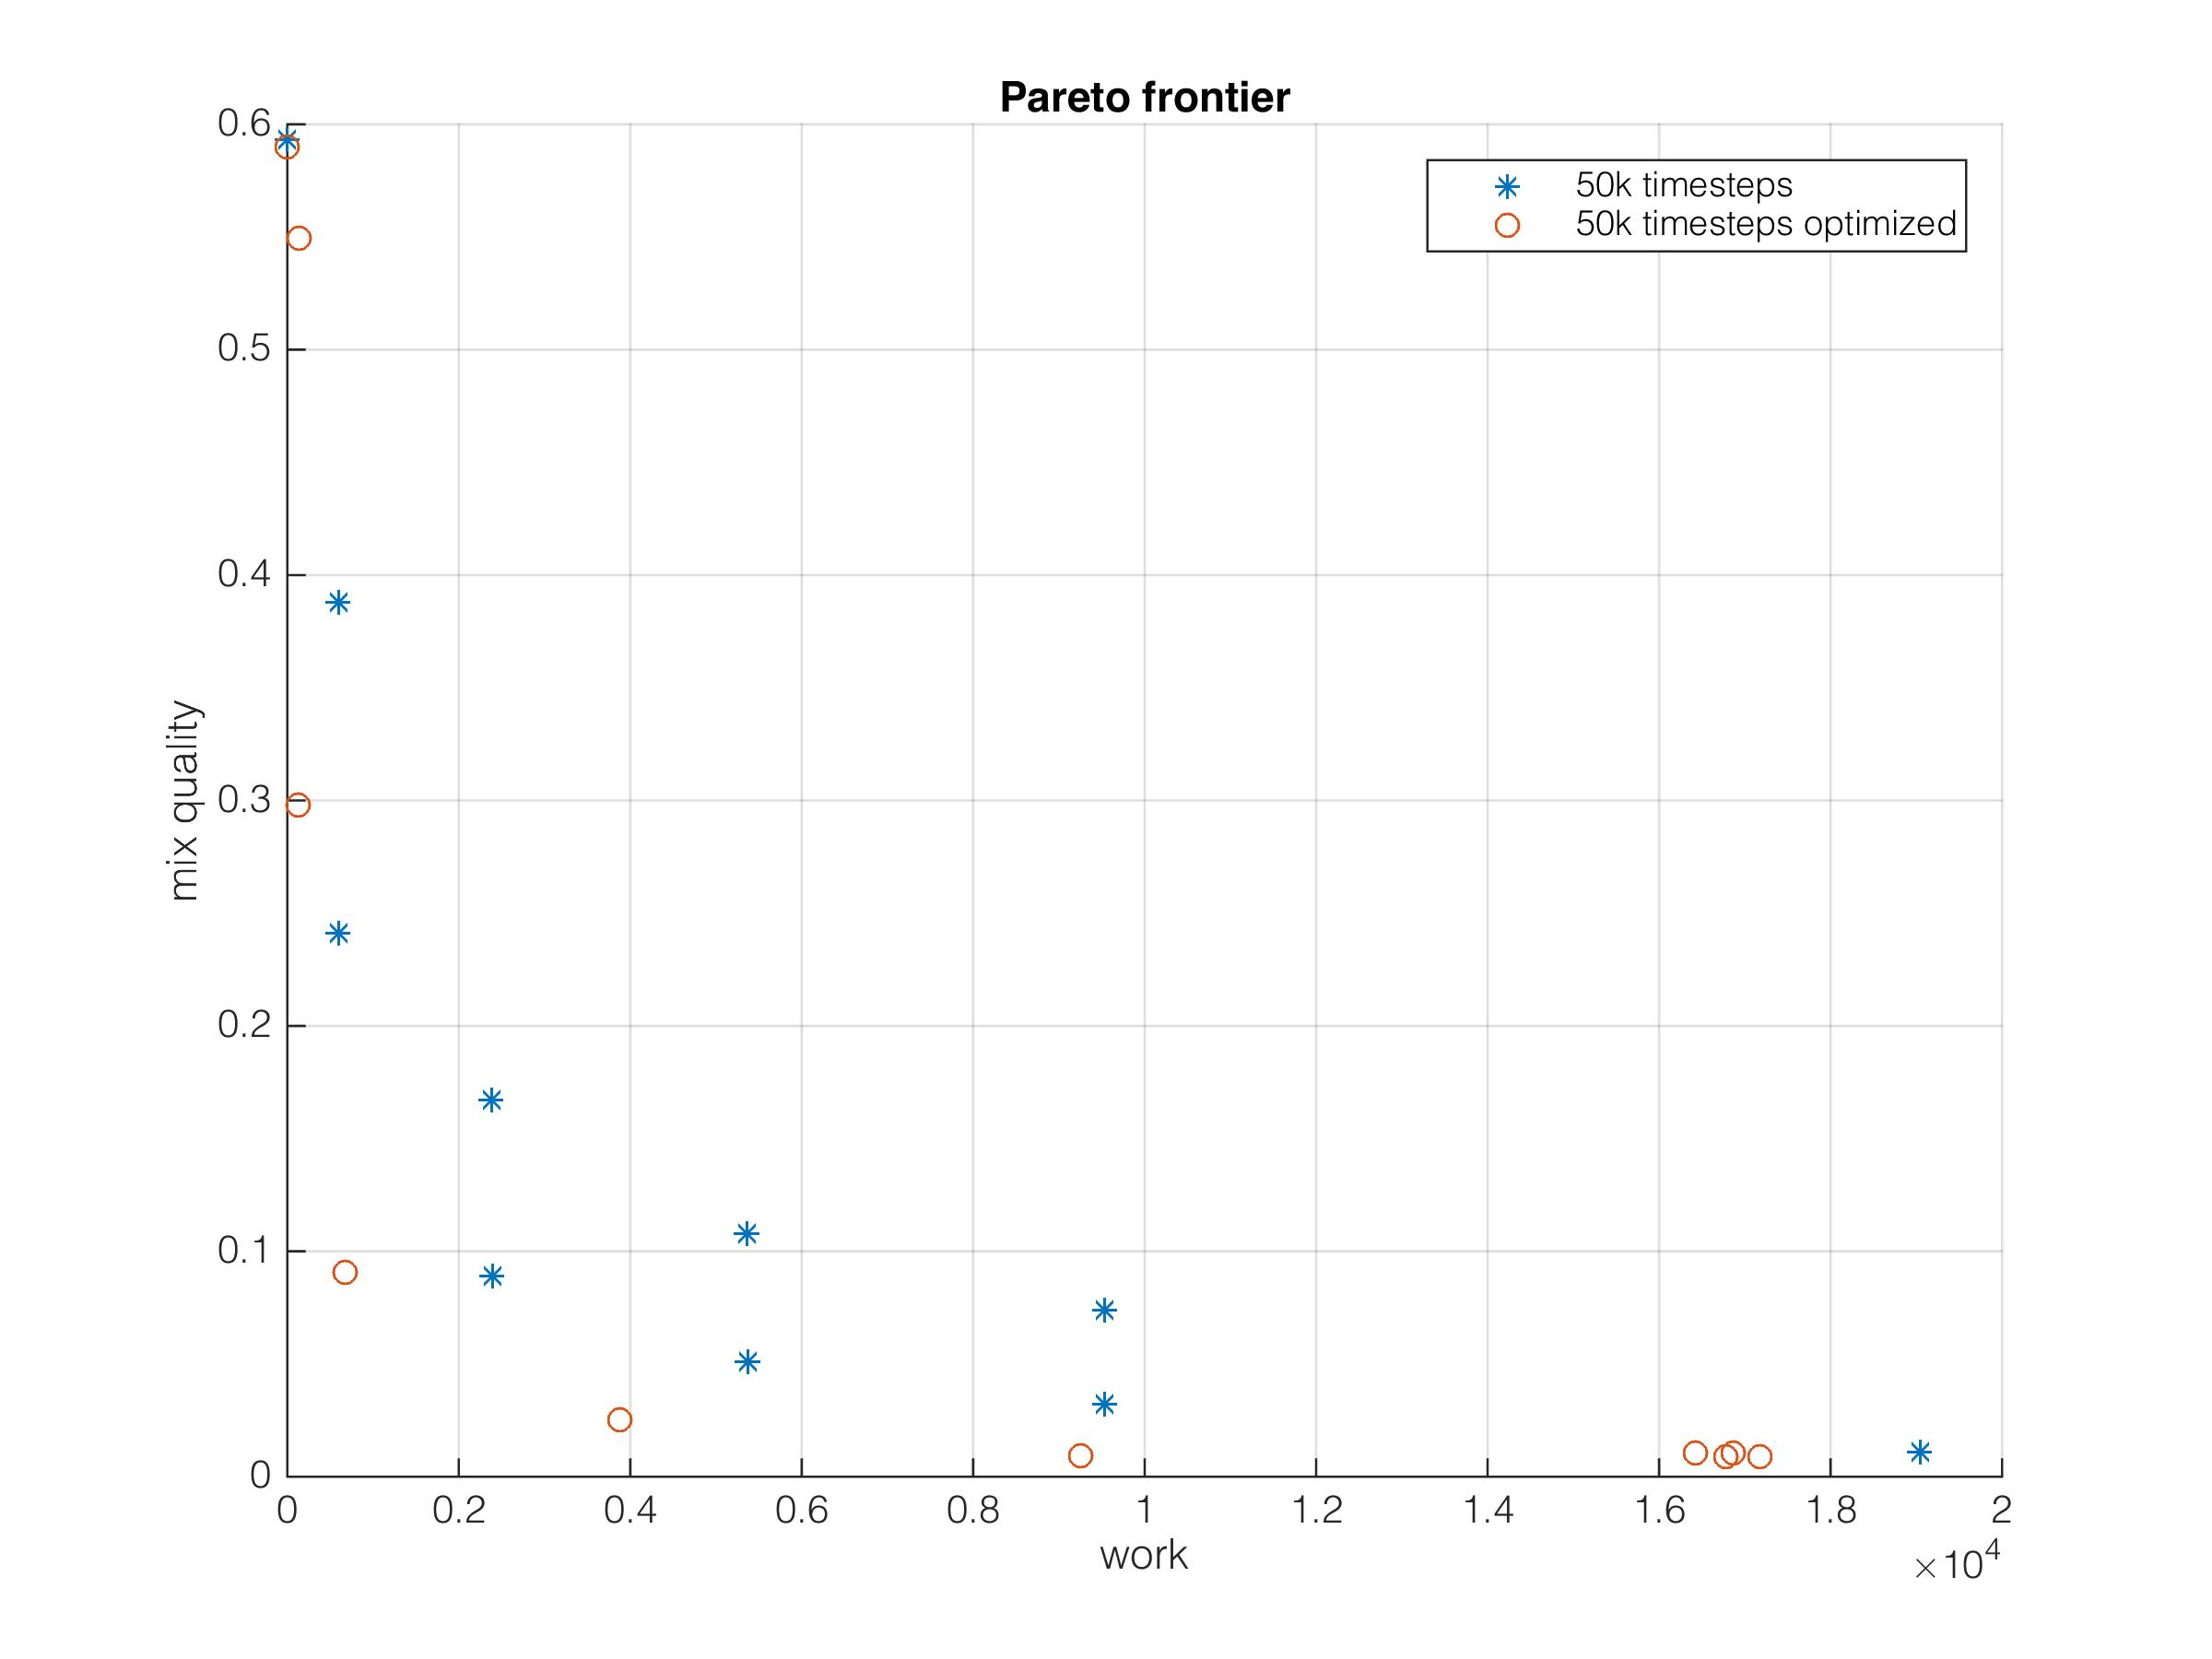
\includegraphics[width=0.9 \textwidth]{obrazki/Pareto_frontier.jpg} 
%\caption{Source Code Transformation}
\end{figure}
\end{frame}

\subsection{Conclusions}
\begin{frame}\frametitle{Conclusions - What we achieved:}

\begin{multicols}{2}
\textbf{Feature:} 
   
\columnbreak
\textbf{Benefits:}
\end{multicols}

\pause
\begin{multicols}{2}
framework for optimization of discrete dynamical system
\columnbreak \\
applicable to complex CFD problems like optimal control or topology optimization
\end{multicols}

\pause
\begin{multicols}{2}
Lattice Boltzmann Method
\columnbreak \\
almost ideal scalability on HPC
\end{multicols}

\pause
\begin{multicols}{2}
adjoint
\columnbreak \\
reduce numerical cost of finding the derivative of the objective depending on many control variables
\end{multicols}

\pause
\begin{multicols}{2}
automatic differentiation
\columnbreak \\
exact derivatives, code maintainability
\end{multicols}

%What we achieved:
%\begin{itemize}
%\item framework for optimization of discrete dynamical system applicable to complex CFD problems like optimal control or topology optimization
%\item adjoint approach - reduces computational cost
%\item LBM  - exhibits almost ideal parallel scalability 
%\item locality of the collision operator
%and reversibility of streaming - allows to utilize the adjoint concept in a parallel manner
%\item automatic differentiation - 
%\end{itemize}
%%%%%%%%%%%%%%%%%%%Future work:
%\begin{tabular}{|c|c|}
%\hline
%\textbf{Method} & \textbf{Why} \\ \hline
%Framework for optimization of discrete dynamical system &  applicable to complex CFD problems like optimal control or topology optimization \\ \hline
%Lattice Boltzmann &  good scalability \\ \hline
%Adjoint &  reduce numerical cost  \\ \hline
%\end{tabular}
\end{frame}

\subsection{Questions?}
\begin{frame}\frametitle{Questions?}

\begin{center}
{\huge ? }
\end{center}
\end{frame}

\appendix
\begin{frame}[t,allowframebreaks]
\frametitle{References}
%\bibliography{<bibfile>}
\printbibliography[title=References]
\nocite {TCLB}
\end{frame}

\end{document}